\documentclass[12pt]{article}
%encoding
\usepackage{fontspec}
%language
\usepackage[english,french]{babel}
%use special characters unicode
\usepackage{xunicode}
\defaultfontfeatures{Ligatures=TeX}
\setmainfont[Numbers=OldStyle]{Junicode}
\usepackage{xspace}
%images and figures
\usepackage{graphicx}
\usepackage{float}
%color tables
\usepackage{colortbl}
\usepackage{xcolor}
%split a table cell in two
\usepackage{diagbox}
\usepackage[style=enc]{biblatex}
 %Imports biblatex package
\addbibresource{biblio/mybibliography.bib} %Import the bibliography file
\usepackage{longtable} %long tables
\usepackage{lscape} %mode paysage
\usepackage{pdflscape}
\usepackage{tabularx}
%images and figures
%new commands
\newcommand{\clearemptydoublepage}{%
	\newpage{\pagestyle{empty}\cleardoublepage}}
%quotations
\usepackage{csquotes}
\renewcommand{\mkbegdispquote}[2]{\itshape}


	
%add hyperlinks
\usepackage{hyperref}
%metadata
\hypersetup{pdfauthor={Matenia Vlachou}{Noé Léroy},pdftitle={report of project-Boccacius-HN2021},pdfsubject={Detailed report and workflow/process of the project for the course "Bonnes pratiques du développement - Git" first semester 2021, university ENC-PSL, prof.Thibault Clérice},pdfkeywords={Boccacius} {De genealogia deorum gentilium} {incunabula} {latin} {middle French} {OCR} {HTR} {e-Scriptorium} {école nationale des chartes} {Master HN 2021}}

\begin{document}

\title{Report of HN-project-Boccacius }
\date{January 2022}
\author{\textsc{Léroy }Noé \and {\textsc{Maulu } Marco}\and {\textsc{Vlachou-Efstathiou } Malamatenia }}

\maketitle

\clearpage

\section{Aknowledgements}

First of all, we would like to thank Professor \textsc{Clérice} Thibault for his valuable help throughout the development of this project. Not only he initiated us in the world of Git and GitHub but he also supported and advised us throughout the procedure in the best way possible, going along with our experimentations and curiosities. A big thank you to Professor \textsc{Pinche} Arianne for her tutorial on eScriptorium, and to both of them as a team for inspiring us with their digital and not only projects. Last but not least, we thank Marco for letting us in his project and consulting us on terms of bibliography and objectives. It was a pleasure kicking off out GitHub activity with such a project that has definitely left us more curious and eager to work.


\section{Project framework}

The starting point of this project was the assignment given to the contributors for the validation of the course Bonnes pratiques du developpement collaboratif : initiation à Git" (prof. Thibault Clérice), for the first semester - Master Humanités Numériques ENC-PSL 2021-2022. It serves, consequently, primarily as to validate the aforementioned course and as an  initiation to the Digital Humanities toolbox.

At the same time, the project is directly linked to, and constitutes part of the biannual project "Per un'edizione digitale della Genealogia deorum gentilium" di Boccaccio" (dir. F. Duval, M. Maulu). Financed in 2021, this project foresees to put on line in XML format the unpublished translation in Middle French entitled "De la genealogie des dieux". The translation in question was published in Paris by A. Vérard in 1498 and probably realized by Laurent Premierfait, which constitutes one of the two main witnessed treated.\\

The basic idea is to exploit the method of treatment and edition developed during the project "Pour une édition numérique de la Mer des histoires" (dir. F. Duval, M. Maulu). Differences between these two projects can already be underlined, notably the choice of EScriptorium instead of Transkribus, which will be analysed thoroughly below. 
It will also be necessary to verify if more efficient tools than http://stella.atilf.fr/LGeRM/glossaire/ can be used in the automatic text correction process. 
Ultimately, the desired outcomes of the Boccace project  are: 
\begin{enumerate}
    \item a decrease in the percentage of error (CER and WER) with a more reliable base text;
    \item  the optimization of a post-HTR processing and correction software
    \item the creation of a new model that can be used for large-scale projects (e.g. a corpus of translations of Latin texts into MF).
\end{enumerate}

The project also includes  the organization of a Summer School in Digital Humanities in Sassari. \\


Although fundamental, a study of the original text in Latin has not been included for budgetary and chronological reasons: compared to the Mdh tradition, which translates a medieval work printed in 1475, the tradition of Boccaccio's work is more extensive.The tradition is exclusively printed and the \textit{editio princeps} is therefore of absolute value ( cf. Hortis \footcite{hortis1879} and Ernest \footcite{ernest1919}) . Given the importance of the author in question and the fact that a true critical edition of \textit{Genealogia} has not been published until now, partial surveys of some of the Latin manuscripts and prints that transmit it could help to understand which textual branch provided the model for the translation published by Vérard.

\clearpage

\section{Presentation and description of document sources}

The data set of the present project consists of two documents, both of them \textit{incunabula}, presented here in chronological order.\\

\subsection{Mazarine Inc.59}

The first one, namely Mazarine \footnote{Abbreviation of the Bibliothèque Mazarine, located in Paris, France.} Inc.59, constitutes the \textit{editio princeps} of the work edited in Venice in 1472\footnote{The document belongs to the public domain.Link to the notice of the library online : https://mazarinum.bibliotheque-mazarine.fr/records/item/1781-genealogia-deorum and to the IIIF manifest:  https://mazarinum.bibliotheque-mazarine.fr/iiif/1781/manifest}. Its format is \textit{in-folio}, numbers 295 folios/leafs, was produced in paper \footnote{for the terminology and the accurate translation from French to English we use the handbook of Denis Muzerelle \textit{Répertoire méthodique
des termes français
relatifs aux manuscrits}, IRHT,CNRS,Paris, available online : http://www.palaeographia.org/vocabulaire/vocab.htm }, measures 322 x 234 x 69 mm and its binding is in case-hardened calf. It was previously owned by Ferdinand I (king of Naples; 1431?-1494) and the
Royal Library of France (15..-1792)
To understand the importance of this document for an eventual critical edition lies to the tradition of the work itself. Its textual tradition is indeed particular, as in 1371 Boccaccio allowed a friend to make a copy of an autograph MS, now lost, of the \textit{Genealogia}, and from that first apograph other copies were made. The text of the lost autograph is now called the Vulgate text which was widely diffused and constituted the base of the editiones made in the !5th and 15th century \footcite{ernest1919}.  This edition contains, first, the Table of Rubrics; second, the Genealogia itself; third, the Alphabetical Index by Domenico Bandini; fourth, the Versus of Domenico di Silvestro. The printer did not undertake to reproduce the genealogical trees which stood presumably in the MS which served him as copy.The edition of 1472 is  the best printed representative of the Vulgate text of the Genealogia, and should be cited, in preference to the edition of 1532, for all portions of the Genealogia, except those printed by Hecker\footcite{hecker1902} from the autograph, and for any citation in which the reading of the Vulgate text as against that of the autograph is desired (More specifically, Hecker prints from the second autograph the Dedicatory Letter (but not the single chapter of the general Proem, nor the Proem of Book I), the Proems of Books II-XIII, and Books XIV and XV entire).
\\ 
\subsection{Rés J-482}

The second manuscript was written in ancient French only a few years after the Venetian \textit{editio princeps}. A previous translation from Latin had been made by Jean Miélot in 1468, but it was fragmentary \footcite{galderisi2014}. The first edited french version was produced in 1498 in Paris by Antoine Vérard. The paternity is proved, because he often signed in the colophon with his name, his address and his printer's mark. The « Rés J-482 » is a great example of this tradition as it concludes as follows : 
 
\begin{displayquote}
 « Cy finist Jehan bocace de la genealogie des dieux. Imprime nouvelleme[n]t a Paris La[n] mil CCCC.quatrevi[n]gtz [et] dixhuit le neufuiesme iour de fevrier. Pour Anthoine verard libraire demourant a Paris sur le pont nostre dame a lymage saint Jehan leva[n]geliste/ ou au palais au premier pilier devant la chapelle ou len chante la messe de messeigneurs les presidens »\footnote{https://www.arlima.net/il/jehan_bocace_de_la_genealogie_des_dieux.html}.
\end{displayquote}


This is the edition we are analyzing for this project since it has never been properly edited after the 19th century. Vérard was the editor, but he was neither the scribe nor the translator of the work. The translation was probably undertaken by Laurent de Premierfait, a French scholar, in the beginning of the century, but only edited a few decades later. Indeed, he was the first French translator of Boccace's texts and he worked on several of them. For example, it is recognized that Vérard published his translation of the Decameron in 1494, a work written between 1414 and 1417\footcite{CarlaBozzolo}. So it is not improbable to deduce that he was also the original translator for the «De la genealogie des Dieux ». 

In total, 15 institutions conserve nowadays a version of this text, mostly in France. This edition is not the most well-documented of all, as shown from the bibliographic record of Gallica\footnote{https://catalogue.bnf.fr/ark:/12148/cb30116914c}. Only the number of folios that compose the manuscript is indicated,namely 226, numbered on the top of each page, and its format : bifolium. Furthermore, the material is not explicitly specified, but can be inferred from another witness made the same year at the same printing center. The « PML 536 » copy, preserved in New York, was compiled on « modern half brown goatskin, with parchment sides, over paper boards »\footnote{https://www.themorgan.org/incunables/133775}.

\clearpage
\section{Tools and Methods}

The two main tools used for the project, other than our personal toil were EScriptorium and GitHub.

\subsection{eScriptorium}

There are plenty OCR (Optical Character Recognition) software : some are proprietary and some are free, and they all have specificities making them more suitable for one project over another.As per the software used for the transcription of Boccacius documents, we used Kraken, through its interface eScriptorium, an OCR system derived from OCRopus, an older OCR system \footnote{Detailed description of the project provided by Professor Peter A. Stokes here : https://www.resilience-ri.eu/blog/resilience-tool-escriptorium/}.

There are two main reasons behind this choice. First of all, it is a well-developed free software with extensive documentation (on an interface \href{https://traces6.paris.inria.fr/}{working interface} and on a GitLab \href{https://gitlab.com/scripta/escriptorium/}{repository}). More specifically, the ENC staff has actively and extensively worked on the project with versions of kraken and eScriptorium and trained models themselves, which means that it was easier fot the team to be trained, to present and resolve issues, be they technical or methodological.

Access to eScriptorium was given from a virtual environment which was fairly easy to navigate and use. It takes on by default the preprocessing steps of binarizing and segmenting the images before performing the transcription, all of this using provided pretrained models, or enabling the user to train customized modeles, as we did for the two documents. The software also offers many options for tailoring the transcription process or the training, depending on the language and layout specificities. 

It is important to note that tools such as eScriptorium, that necessitate a complex preparation of the documents in order to give quality results, may not be worth the effort  applying on one short document, or a number of heterogeneous documents (that are all written with very different scripts or layouts). On the other hand, as it was the case for \textit{Mazarine Inc.59} and \textit{BnF. Rés. J-845} for large and relatively coherent \textit{corpus}, then this software is very useful as it  automatises the process of transcription.

Of course, using artificial intelligence and trained models does not mean that the documents are magically transcribed with impeccable accuracy, which means that a manual supervised - and/or philological- correction of the transcription is necessary. More will be discussed on the process, difficulties and limits for the models trained by the team for this project later.


\subsection{GitHub}

GitHub\href{https://github.com/} is an easily accessible open-source repository, sort like a cloud for code. It hosts source code projects of any kind and keeps track of the changes made. Repositories are public, which means that other GitHub users can review and propose changes to a code via three basic processes: \texttt{fork}, \texttt{push}, \texttt{pull requests}that can be manipulated either from the terminal or from the interface itself. Proposed changes can be merged into the software after the proposals/issues are reviewed and approved. This means that we had a powerful tool to work collaboratively and add progressively to  our work while keeping track of the process. Our personal organisation hosting the Boccacius project is called Boccacius - De genealogia deorum gentilium and its repository can be found here \href{https://github.com/HN-2021-Boccacius/git-project-Boccace}.

A defining feature of GitHub the version control system, accessible, between others, though GitHub Actions. The version control allows developers to establish a workflow,  and potentially fix bugs or improving efficiency without affecting the software itself. For all these reasons, GitHub was the appropriate platform to test out our collaborative skills and track the history of our work, all while establishing workflows to ensure the quality of our data.

\clearpage
\section{Mazarine Inc. 59}

Passing on to the individual process of preparation, segmentation and transcription of the documents, starting with the \textit{editio princeps}.

\subsection{Segmentation process,norms and limits}

The documents, given that is a well curated print, did not pose insurmountable difficulties with the layout. Some features taken into consideration for the training of the segmentation model were:
\begin{enumerate}
    \item The division of the page into columns, applicable only to the first 20 pages that present the "Table of content". The model was trained to read the columns one by one vertically, instead of each line horizontally.
    \item  The posterior addition of the \textit{foliation} (page numbering) in arabic numerals on the top right of each \textit{recto} of the \textit{bifolio}. The lighter -comparing to the main text- ink  made it difficult for recognizing the foliation at the start. At this point it is important to note that the text was divided into two \textit{regions}, the main text (capital initials included) and the page numbering and while exporting the text only these two labels were chosen.
    \item The initial capitals. It was particularly tricky to train the machine into recognizing the initial letters for two reasons. Firstly, as expected, they do not precede the line that normally follows the same baseline but a previous line (usually wither one or two levels above). Secondly, they are often times omitted, which means that there is a space left. These two factors made it impossible to integrate them into a full line with their complement, and imposed a separate line for the initials that would then be re positioned prior to the corresponding line. 
    An additional problem was the printing of the capitals in a second time over the corresponding minuscule letters that indicate where the capitals should be placed. 
 \end{enumerate}   
 
\begin{figure}[h!]
    \centering
    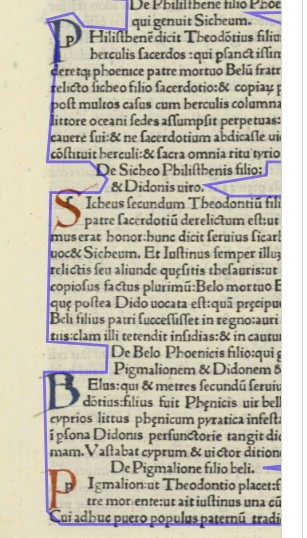
\includegraphics[width=5cm]{initial_capitals.jpg}
    \caption{Overwritten initals}
    \label{fig:PremFigure}
\end{figure}


This being said, since eScriprotium recognizes characters, and for this case one should eliminate the other, it was proved to be a fastidious task for the training procedure and was eventually corrected by hand in all cases.


\subsection{Transcription process,norms and limits}
A valuable guide was that of Capelli \footcite{cappelli1982elements} in order to verify the abbreviation and ligature system used in the \textit{incunabulum}/print.\\

\begin{landscape}

\pagestyle{empty}

%creating my special characters commands
\newcommand{\rum}{\char"A75D\xspace}
\newcommand{\pro}{\char"A753\xspace}
\newcommand{\per}{\char"A751\xspace}
\newcommand{\eced}{\char"0119\xspace}
\newcommand{\quod}{\char"A759\xspace}
\newcommand{\Quod}{\char"A756\xspace}
\newcommand{\ussup}{\char"1DD2\xspace}
\newcommand{\pre}{\char"A751\xspace}
\newcommand{\macron}{\char"0303\xspace}
\newcommand{\ursup}{\char"1DD1\xspace}
\newcommand{\opena}{\char"1DD3\xspace}
\newcommand{\qu}{\char"A757\xspace}
\newcommand{\isup}{\char"0365\xspace}
\newcommand{\etc}{.2c\opena{}.\xspace}
\newcommand{\sm}{\char"1E9C{}m\xspace}


\begin{table}[!h]
\centering
\begin{tabularx}{\textwidth}{| X | X | X |X|}\hline
\textsc{Abbreviation}     & \texttt{mufi unicode} (if applicable)    & \textsc{special character sign}  & \textsc{examples} \\ \hline\hline
omission of macron & 0303 & \macron{} & e\macron{} a\macron{} i\macron{} m\macron{}etc. \\\hline
ligature of est & - & e\macron{}& \\\hline
ligature of esse & - & ee\macron{} & \\\hline
open a superscript & 1DD3 & \opena{} & q\opena{} \\\hline
-rum        & A75D     & \rum{}   or 4 & re\rum{} \\ \hline
-i superscript &  0365 & \isup{} & \qu{}\isup{}, p\isup{}  \\\hline
-ur superscript & 1DD1 & \ursup{} & t\ursup{} \\\hline
-ae &  0119 & \char"0119 &\\\hline
Abbreviation of -us / 9 superscript & IDD2 & \ussup{} & r\ussup{}\\\hline
suffix pro & A753 & \pro{} & \pro{}ducta \\\hline
suffix per & A751 & \pre{} & \per{}crutat\ursup{} \\\hline
Abbreviation of quod & A759 & \quod{} & \\\hline
Abbreviation of Quod & A759 & \Quod{} & \\\hline
abbreviation of qu (+ macron) & A757 & \qu{} & tran\qu{}litatem  \\\hline
Ligature of quam & A757 + 1DD3 & \qu{}\opena{} & tam\qu{}\opena{}, um\qu{}\opena{} \\\hline
abbreviation of etcaetera & - & \etc{} \footnote{Replacing the tironian textit{et} with 2 because in this case it represents better the representation of the sign. The tironian "and" is never found isolated in the document.} & \\\hline
abbreviation of \textit{secundum} & 1E9C + m & \sm{}& \\\hline
\end{tabularx}

\caption{\textsc{Transcription guidelines. Table of special character signs}}
\label{table:1}
\end{table}

\end{landscape}

With these conventions in hand, that serve as out base and cover, in combination or not, all of the signs witnessed in the document \footnote{At least on the fist 27 pages that were transcribed and corrected for the project. In any new characters that this table does not satisfy, solutions should be given in the mufi unicode site.} can be transcribed without problem. The use of the signs is not regular and abbreviated forms are used interchangeably with the developed ones, according to the layout and the space line management. for example qui and \char"A757 , omission of macrons etc.

In general the transcription is completely graphemic, according to which a sign in the image corresponds to a sign in the transcription. Furthermore, u/v or i/j are not distinguished and transcriptions reproduce the exact manuscript spacing and signaling (space for modern spacing, : for modern commas and . between numbers and at the and of a phrase).
Orthography is by no means corrected, but philological intervention was necessary (but fortunately limited) to the letters that are inverted, almost all of the cases \footnote{There is one case of an inverted "t" in the word \textit{Cocyto} in page 4 that was correctly transcribed. Other common instances where the u was inverted are \textit{quorum}, \textit{coniuge} and \textit{genuit}. } a u inverted, giving an n, as seen in the example below:

\begin{figure}[!h]
    \centering
    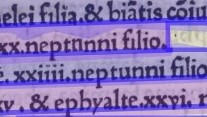
\includegraphics[width=5cm]{neptunni.jpg}
    \caption{Two instances of the genitive \textit{neptunni} , one with a reversed u and one corrected.}
    \label{fig:SecFigure}
\end{figure}
In case of doubt over a given word, the transcriber verified if the form exists or not via the Collatinus lemmatiser \hyperref[Collatinus]{https://outils.biblissima.fr/fr/collatinus-web/} before the correction.

For the training of the model for the transcription the procedure was the following:
First, the 20 first pages (10 folios) were transcribed manually, and constituted the initial corpus of training. They were progressively inserted to the model 5, giving respectively 4 pages of verification. These 4 pages were then corrected manually and were reinserted to the model (fine-tuning). Lastly, another 3 pages were corrected and added to the model with the same method, which gave a very satisfying outcome and an accuracy level of 97\%.
\begin{figure}[!h]
    \centering
    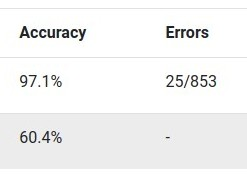
\includegraphics[width=5cm]{training_status.jpg}
    \caption{The training status of the recognition and segmentation models respectively.}
    \label{fig:ThirdFigure}
\end{figure}

Automatic transcription is not magic and a certain number of recurrent errors was observed.
\begin{figure}[!h]
    \centering
    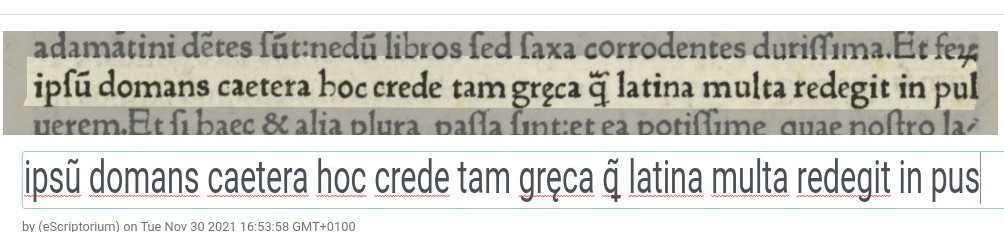
\includegraphics[width=10cm]{good_transcription.jpg}
    \caption{In some cases, the transcription is quasi perfect.}
    \label{fig:SecFigure}
\end{figure}

Namely, 
\begin{enumerate}
    \item the fist or last line of the document is almost always filled with errors, even if the ones that follow are more or less accurate;
    \item \textit{idem} with the first or last letter of every line, depending on how well the lines are designated during segmentation.
    \item double consonants or vowels are reduced to one instead of two;
    \item omission of the "i" in the particle \textit{si};
    \item open s, the letter f and the first component of the abbreviation of \textit{secundum} (\char"1E9C m) are sometimes confused;
    \item \textit{idem} for the letters b and h;
\end{enumerate}

This means that assisted post correction is needed for the most part, a statement that does not nevertheless undermine the overall efficiency of the model, as the time of transcription has been significantly reduced.


\section{BnF. Rés. J-845}
\subsection{Segmentation process,norms and limits}

First of all, the final segmentation presents different types of zones - regions. All things considered, there are four zones to be determined. Each page has two main columns of text surrounded by marginal annotations. The title is repeated one out of two pages but was not considered for the purpose of this research. But, on the other hand, the mention of the leaflets and their enumeration, also indicated on the top of the page, are all included in a zone named « feuillets ».All these features are distinguishable on the figure that follows. To the zones mentioned previously, we added initials for practical reasons. We witnessed two possible outcomes : first case scenario, the automatic segmentation only rarely included those letters : second case scenario, the automatic segmentation put the initial in more than one line, which was not efficient for the transcription. In the end, manual adjustments, minor or not had to be made in order to properly align the text but a significant amount of time is saved by using the model. 
´
\begin{figure}[h!]
    \centering
    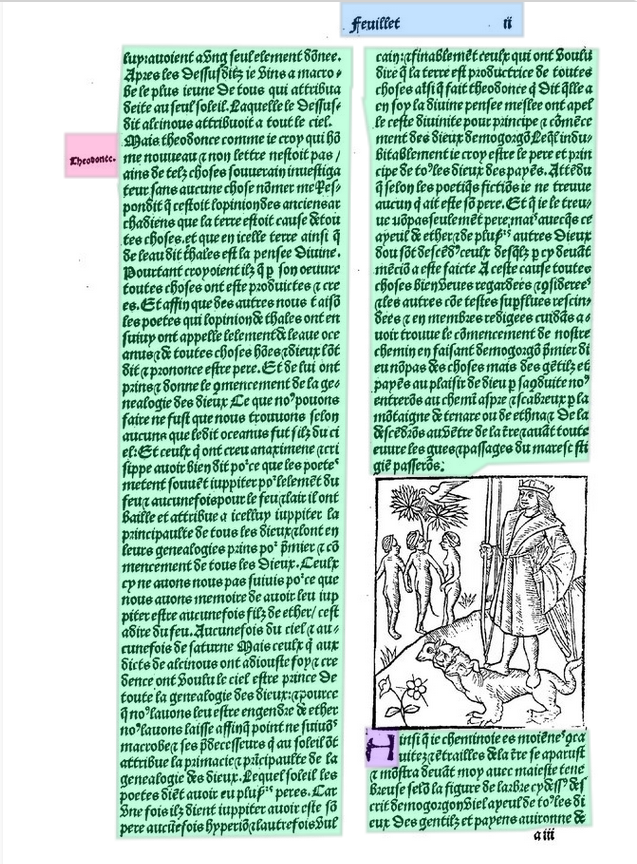
\includegraphics{Page escriptorium.png}
    \caption{Layout of the zones from e-scriptorium}
    \label{fig:3}
\end{figure}

Other modifications to the automatic segmentation had to be made. For instance, it sometimes occurred that lines were not accurate enough and had to be reassigned or deleted. Also, the lines in the marginal notes did not allow us to define the area of the main text, and had to be deleted and recreated manually so they wouldn't interfere with the main text. Similarly, the zones delimited by the the model did not always include the lines from start to end : the same approach was thus applied (suppression or reassignment) to the incomplete zones.


We used a sample of twenty pages (10 folios) for the training of the A.I. and obtained a result of 66 percent of accuracy. This model can surely be optimized, but due to time restrictions, it shall not be included in the framework of this project. Although we do recognise the liability of the percentage remains of the lower side, we believe that the model is functional enough to partially recognize all the zones. The model is limited and has yet to improve, but we believe it has potential as it already decreases the amount of time that it takes to segment the text.

\subsection{Transcription process,norms and limits}

As for the transcription part, we focused mainly around the norms of transcription. We had to ask ourselves: how do we retain as much  information as possible from the original text ? The text was mostly spaced, but on few occasions, words were attached to one another We decided to separate the words were attached, so that if a lemmatisation step was planned, it would ease the workload and the reprocessing. Some word forms were kept untouched when not understood. Additionally, we also had to find a way to render the abbreviations- which were numerous, but not omnipresent. Nevertheless they are regular. We focused our attention to the list available on Ariane Pinche’s project : HTR-United : cremma medieval (link to the github repository : https://github.com/HTR-United/cremma-medieval/blob/main/table.csv\#L116). The most frequent ones are referred to in the second table. 

\begin{table}[!h]
\centering
\begin{tabularx}{\textwidth}{| X | X | X |}\hline
\textsc{Abbreviation}     & \texttt{Cremma code} (if applicable)    & \textsc{special character sign}  \\ \hline\hline
Combining tilde & 16 & ̃  \\\hline
Tironian et & 48 & 2 & \\\hline
Ligature of a word between two lines & 35 & “ & \\\hline
-s superscript & 165 & ˢ \\\hline
-i superscript &  110 & ͥ \\\hline
-ur superscript & 20 & ᷑ \\\hline
er/re & 18 & ̾\\\hline
Abbreviation of -us / 9 superscript & 200 & ꝰ \\\hline
suffix pro & 151 & ꝓ \\\hline
suffix per & 17 & ̄  \\\hline
abbreviation of "que" (+ macron) & 17 & ̄  \\\hline

\end{tabularx}

\caption{\textsc{Transcription guidelines. Table of special character signs for the French transcription}}
\label{table:1}
\end{table}

The training method that we followed consisted of manually transcribing the first 20 pages (10 folios). The actual training process was done in five consecutive stages: we trained a model from the five first pages, which wasn't very conclusive. But from this model draft, we retrained the A.I. with 3 more pages (fine-tuning), and continued this process until we had integrated every single page. The result speaks for itself : we obtained a final model with 96.1\% accuracy. 

Still, there is a remark to make. During this process of machine learning, the result wasn't always improving, it sometimes regressed (a certain plateau was reached). That's why we decided to save the second most effective model as well, in order to show the evolution process. A 96.4\% model was created, but unfortunately erased in the making. Nevertheless, each model from each step was tested on a random page from the edition and shows the improvements and the worsening of our work. They all can be found on our Github repository, in a folder named "Validation corpus". 


\section{Re-framing the project and collaboration perspectives}

The instructions for this report indicated that we had to plan the eventual integration of a new member in the work group or an external collaborator. This was taken into consideration in a certain way. Indeed, the project itself started out as a collaboration between the three members of the group and the workflow was built that way in order to facilitate external manipulation of the data-set. One member worked on the Latin version, as explained above in order to get familiar with the original tradition and establish the specific guidelines for the transcription, and the second member worked on the french translation.

The clear description and the indications given by the members can allow two things at the same time: verify the quality of the transcriptions provided by the team members by iterating their procedures and secondly, contribute to the project itself by transcribing the remaining incunabula independently.

A part the specific \textit{incunabula} the whiteness tradition is abundant and it's only through a collaborative approach that can be tackled effectively. This way,a new member could join the team - preferably a specialist-  and dedicate himself to the segmentation and transcription of another manuscript from the Latin tradition following the already existing workflow. In this context, he could use the tools we created and accelerate his transcription with the help of our models. But, he could also contribute and improve any procedure by confronting new and old materials.

The HTR United framework from which the project drew upon already tries to establish a collaborative way of transcribing manuscripts by democratising pre-trained models with the ground truth in order facilitate transcription procedures and implementation of new texts by fine-tuning these existing models. We adhere to their mindset and propose our own ground truth for Boccace's \textit{De genealogia deorum gentilium}.

Something that really distinguishes HTR is the fact that its developers (Professor Clérice) have provided  their project with quality control tools. Chocomufin is a software-workflow developped by Clérice Thubault and Pinche Ariane that creates a table of the characters (```table.csv```) that exist in the ground truth for both documents, and checks, with every push and pull request that the .xml documents found in the folders are conforming to this particular table. This approach guarantees the control of every file that enters the repository, the sustainability and homogeneity of the transcriptions.More information and details about the HTR initiative see. the latest article published by Chagué Alix and Clérice Thibaut \footcite{chagueclerice2021}. 

\clearpage

\tableofcontents
%
\printbibliography
%

\end{document}
\documentclass[12pt,twoside]{article}

